\documentclass{article}
\usepackage{amsmath}
\usepackage{amssymb}
\usepackage{graphicx}
\usepackage{hyperref}
\usepackage[version=4]{mhchem}


\begin{document}
(AMC) Vertex \(E\) of equilateral triangle \(A B E\) is in the interior of square \(A B C D\), and \(F\) is the point of intersection of diagonal \(B D\) and line segment \(A E\). If length \(A B\) is \(\sqrt{1+\sqrt{3}}\) then the area of \(\triangle A B F\) is\\
(A) 1\\
(B) \(\frac{\sqrt{2}}{2}\)\\
(C) \(\frac{\sqrt{3}}{2}\)\\
(D) \(4-2 \sqrt{3}\)\\
(E) \(\frac{1}{2}+\frac{\sqrt{3}}{4}\)\\
\centering
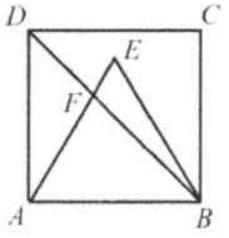
\includegraphics[width=\textwidth]{images/083.jpg}

Solution: (C).\\
Let \(F G\) be an altitude of triangle \(A B E\), and let \(x\) denote the length of \(A G\). From the adjoining figure it may be seen that

\[
\begin{aligned}
\sqrt{1+\sqrt{3}} & =A B=x(1+\sqrt{3}) \quad \Rightarrow \quad 1+\sqrt{3}=x^{2}(1+\sqrt{3})^{2} \quad \Rightarrow \\
1 & =x^{2}(1+\sqrt{3})
\end{aligned}
\]

\begin{center}
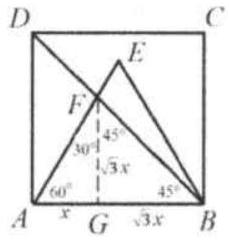
\includegraphics[width=\textwidth]{images/083(1).jpg}
\end{center}

The area of triangle \(A B E\) is \(\frac{1}{2}(A B)(F G)=\frac{1}{2} x^{2}(1+\sqrt{3}) \sqrt{3}=\frac{\sqrt{3}}{2}\).\\

\end{document}
